% This LaTeX was auto-generated from MATLAB code.
% To make changes, update the MATLAB code and export to LaTeX again.

\documentclass{article}

\usepackage[utf8]{inputenc}
\usepackage[T1]{fontenc}
\usepackage{lmodern}
\usepackage{graphicx}
\usepackage{color}
\usepackage{hyperref}
\usepackage{amsmath}
\usepackage{amsfonts}
\usepackage{epstopdf}
\usepackage[table]{xcolor}
\usepackage{matlab}

\sloppy
\epstopdfsetup{outdir=./}
\graphicspath{ {./calculation_images/} }

\begin{document}

\matlabheadingtwo{Part 1}


\vspace{1em}
\begin{par}
\begin{flushleft}
Input Signal
\end{flushleft}
\end{par}

\begin{matlabcode}
time = 0:1e-7:5e-5;
ip = 0.05*sin(2*pi*100e3*time);
figure()
plot(time,ip)
grid("on")
title("I/P: Sine wave (f=100kHz, Amp=0.05V)")
xlabel('Time (s)')
ylabel('Amplitude (V)')
xlim([0,5e-5]);
\end{matlabcode}
\begin{center}
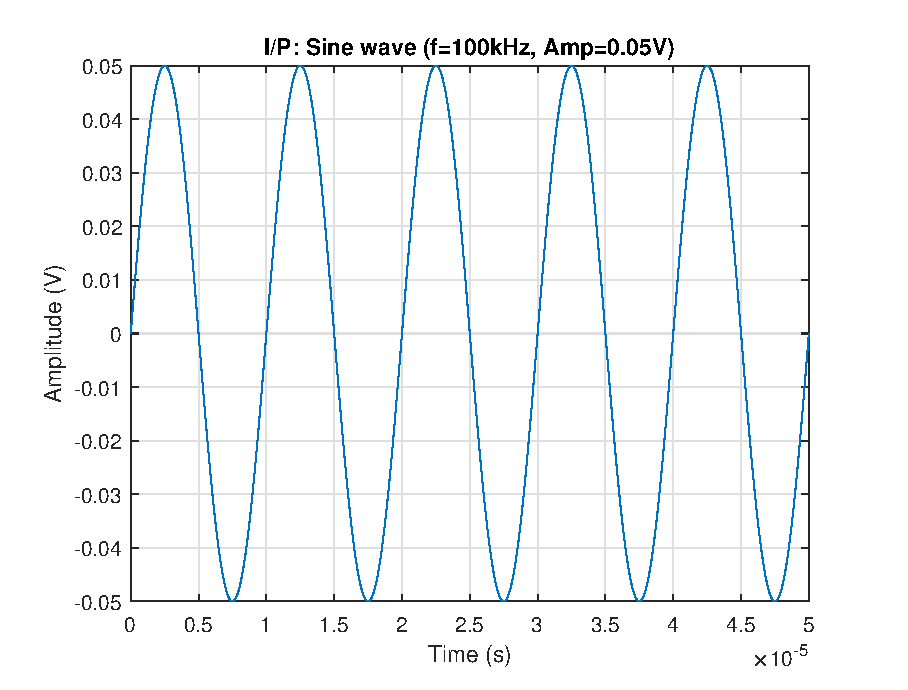
\includegraphics[width=\maxwidth{56.196688409433015em}]{figure_0.eps}
\end{center}


\vspace{1em}
\begin{par}
\begin{flushleft}
Analysis
\end{flushleft}
\end{par}

\begin{matlabcode}
figure()
set(gcf,'Position',[0,0,1000,1000])
T1 = readtable("part1.xlsx");
t = tiledlayout(3,3);

nexttile
plot(T1.t1, T1.D1)
title("f=20kHz")
grid("on")
%xlim([0, 4e-5]);
%ylim([-0.05, 0.05]);

nexttile
plot(T1.t2, T1.D2)
title("f=50kHz")
xlim([0, 4e-5]);
grid("on")
%ylim([-0.05, 0.05]);

nexttile
plot(T1.t3, T1.D3)
title("f=100kHz")
xlim([0, 4e-5]);
grid("on")
%ylim([-0.05, 0.05]);

nexttile
plot(T1.t4, T1.D4)
title("f=200kHz")
xlim([0, 4e-5]);
ylim([-0.05, 0.05]);
grid("on")

nexttile
plot(T1.t5, T1.D5)
title("f=500kHz")
xlim([0, 4e-5]);
ylim([-0.05, 0.05]);
grid("on")

nexttile
plot(T1.t6, T1.D6)
title("f=1MHz")
xlim([0, 4e-5]);
ylim([-0.05, 0.05]);
grid("on")

nexttile
plot(T1.t7, T1.D7)
title("f=2MHz")
xlim([0, 4e-5]);
ylim([-0.05, 0.05]);
grid("on")

nexttile
plot(T1.t8, T1.D8)
title("f=5MHz")
xlim([0, 4e-5]);
ylim([-0.05, 0.05]);
grid("on")

nexttile
plot(T1.t9, T1.D9)
title("f=10kHz")
xlim([0, 4e-5]);
ylim([-0.05, 0.05]);
grid("on")

title(t,'Experimental Verification of Nyquist criterion')
ylabel(t,'Amplitude (V)')
xlabel(t,'Time (s)')
\end{matlabcode}
\begin{center}
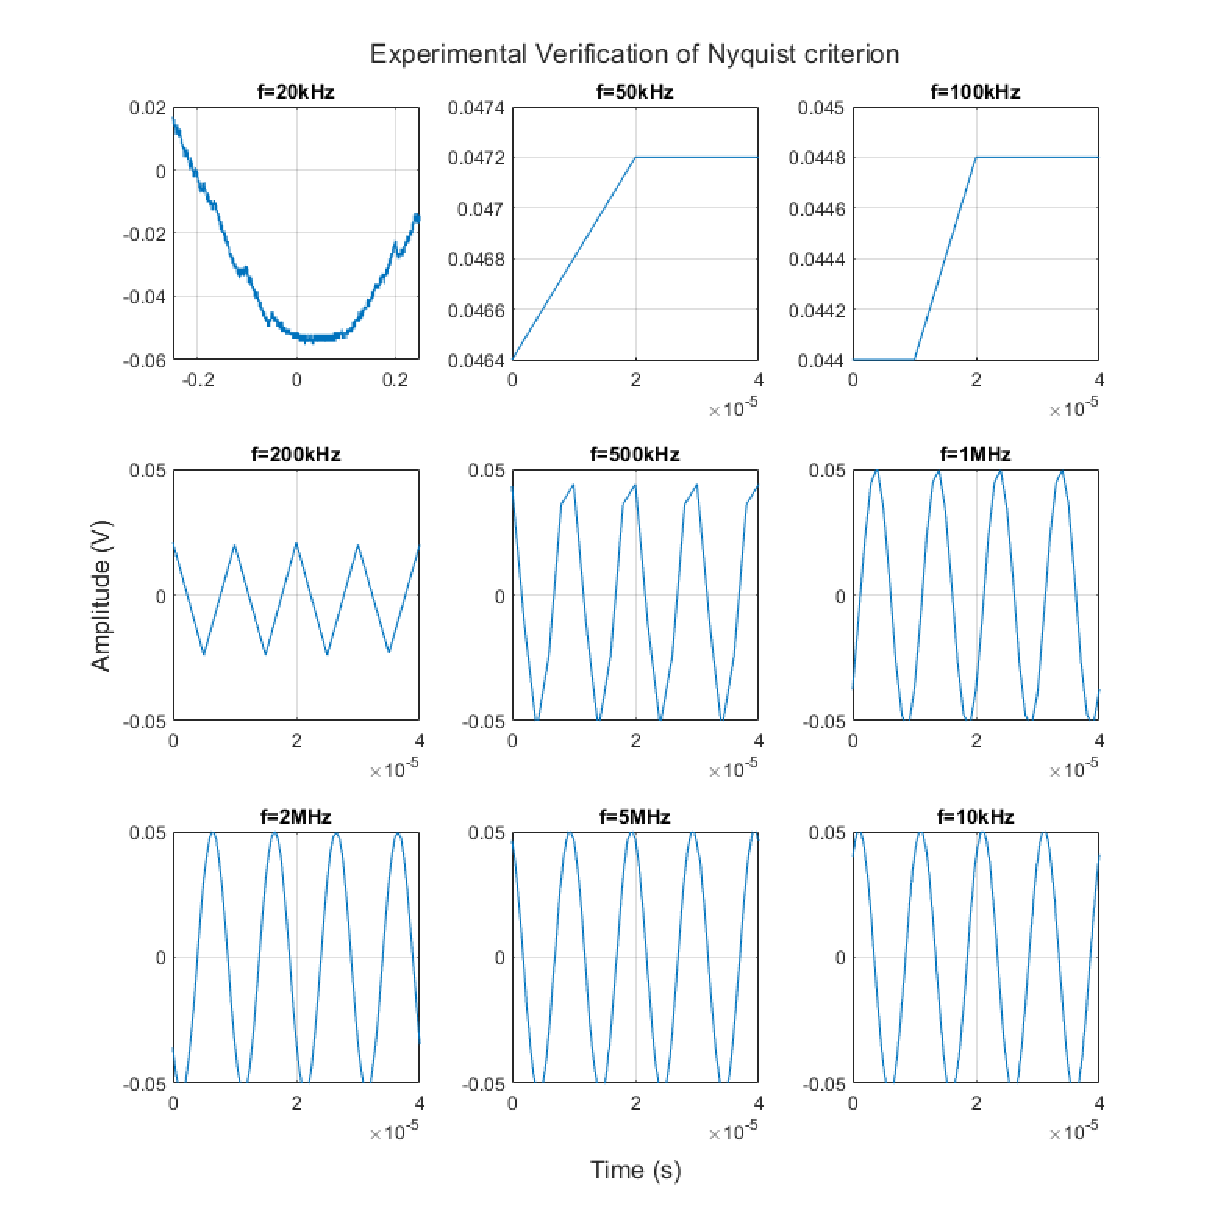
\includegraphics[width=\maxwidth{80.28098344204717em}]{figure_1.eps}
\end{center}

\matlabheadingtwo{Part 2}

\begin{par}
\begin{flushleft}
Input Signal
\end{flushleft}
\end{par}

\begin{matlabcode}
time = 0:1e-7:5e-5;
ip = 0.05*sawtooth(2*pi*100e3*time);
figure()
plot(time,ip)
grid("on")
title("I/P: Sawtooth wave (f=100kHz, Amp=0.05V)")
xlabel('Time (s)')
ylabel('Amplitude (V)')
xlim([0,5e-5]);
\end{matlabcode}
\begin{center}
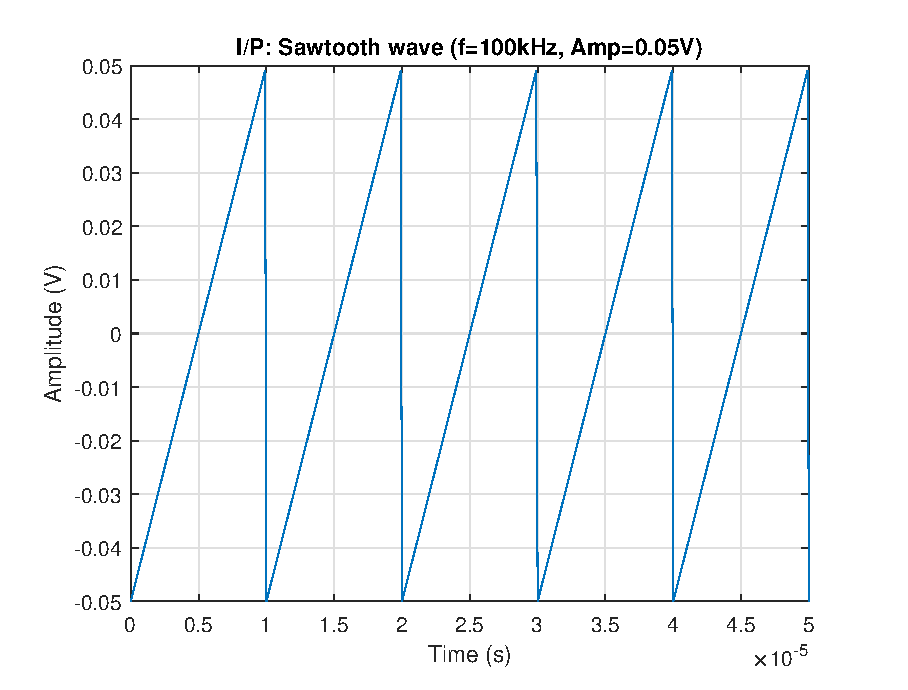
\includegraphics[width=\maxwidth{56.196688409433015em}]{figure_2.eps}
\end{center}

\begin{par}
\begin{flushleft}
Finding the best resolution
\end{flushleft}
\end{par}

\begin{matlabcode}
T2 = readtable("part2.xlsx");
figure()
t = tiledlayout(2,2);
nexttile
plot(T2.t10, T2.D10)
title("Resolution=20mV")
grid("on")
xlim([0, 5e-5]);
ylim([-0.06, 0.06]);

nexttile
plot(T2.t11, T2.D11)
title("Resolution=50mV")
grid("on")
xlim([0, 5e-5]);
ylim([-0.06, 0.06]);

nexttile
plot(T2.t12, T2.D12)
title("Resolution=100mV")
grid("on")
xlim([0, 5e-5]);
ylim([-0.06, 0.06]);

nexttile
plot(T2.t13, T2.D13)
title("Resolution=200mV")
grid("on")
xlim([0, 5e-5]);
ylim([-0.06, 0.06]);

title(t,'Effect of varying the data-resolution')
ylabel(t,'Amplitude (V)')
xlabel(t,'Time (s)')
\end{matlabcode}
\begin{center}
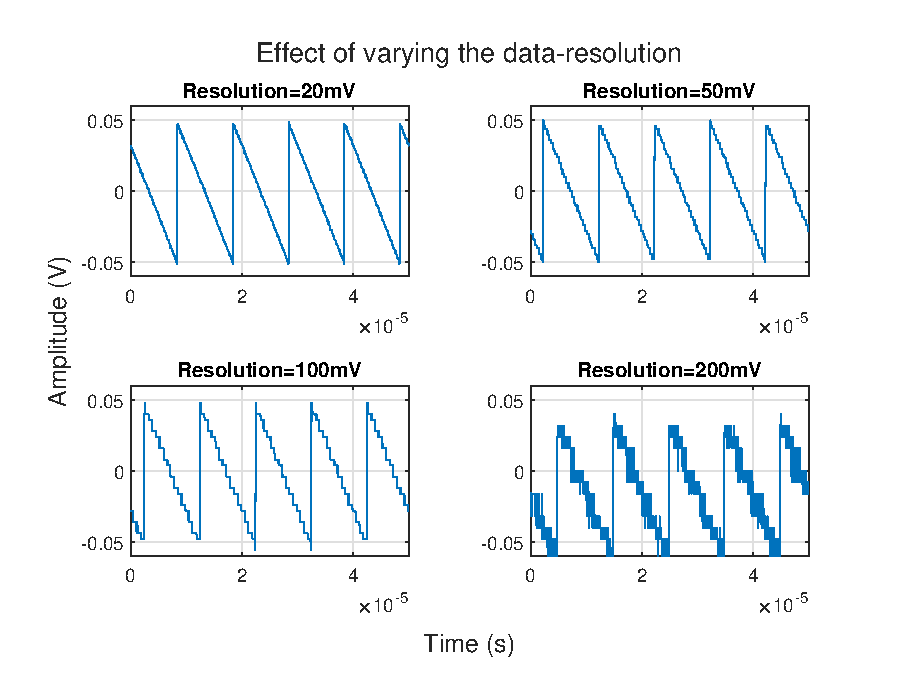
\includegraphics[width=\maxwidth{56.196688409433015em}]{figure_3.eps}
\end{center}


\vspace{1em}
\matlabheadingtwo{Part 3}

\begin{matlabcode}
T3 = readtable("part3.xlsx");
figure()
set(gcf,'Position',[0,0,1000,1600])
t = tiledlayout(5,3);
nexttile
plot(T3.t14, T3.D14)
title("f=20kHz")
grid("on")
xlim([0, 5e-6]);
ylim([-0.05, 0.05]);

nexttile
plot(T3.t15, T3.D15)
title("f=50kHz")
grid("on")
xlim([0, 5e-6]);
ylim([-0.05, 0.05]);

nexttile
plot(T3.t16, T3.D16)
title("f=100kHz")
grid("on")
xlim([0, 5e-6]);
ylim([-0.05, 0.05]);

nexttile
plot(T3.t17, T3.D17)
title("f=200kHz")
grid("on")
xlim([0, 5e-6]);
ylim([-0.05, 0.05]);

nexttile
plot(T3.t18, T3.D18)
title("f=500kHz")
grid("on")
xlim([0, 5e-6]);
ylim([-0.05, 0.05]);

nexttile
plot(T3.t19, T3.D19)
title("f=1MHz")
grid("on")
xlim([0, 5e-6]);
ylim([-0.05, 0.05]);

nexttile
plot(T3.t20, T3.D20)
title("f=2MHz")
grid("on")
xlim([0, 5e-6]);
ylim([-0.05, 0.05]);

nexttile
plot(T3.t21, T3.D21)
title("f=5MHz")
grid("on")
xlim([0, 5e-6]);
ylim([-0.05, 0.05]);

nexttile
plot(T3.t22, T3.D22)
title("f=10MHz")
grid("on")
xlim([0, 5e-6]);
ylim([-0.05, 0.05]);

nexttile
plot(T3.t23, T3.D23)
title("f=20MHz")
grid("on")
xlim([0, 5e-6]);
ylim([-0.05, 0.05]);

nexttile
plot(T3.t24, T3.D24)
title("f=50MHz")
grid("on")
xlim([0, 5e-6]);
ylim([-0.05, 0.05]);

nexttile
plot(T3.t25, T3.D25)
title("f=100MHz")
grid("on")
xlim([0, 5e-6]);
ylim([-0.05, 0.05]);

nexttile
plot(T3.t26, T3.D26)
title("f=200MHz")
grid("on")
xlim([0, 5e-6]);
ylim([-0.05, 0.05]);

nexttile
plot(T3.t27, T3.D27)
title("f=500MHz")
grid("on")
xlim([0, 5e-6]);
ylim([-0.05, 0.05]);

nexttile
plot(T3.t28, T3.D28)
title("f=1GHz")
grid("on")
xlim([0, 5e-6]);
ylim([-0.05, 0.05]);

title(t,'Unknown signal at different sampling frequency')
ylabel(t,'Amplitude (V)')
xlabel(t,'Time (s)')
\end{matlabcode}
\begin{center}
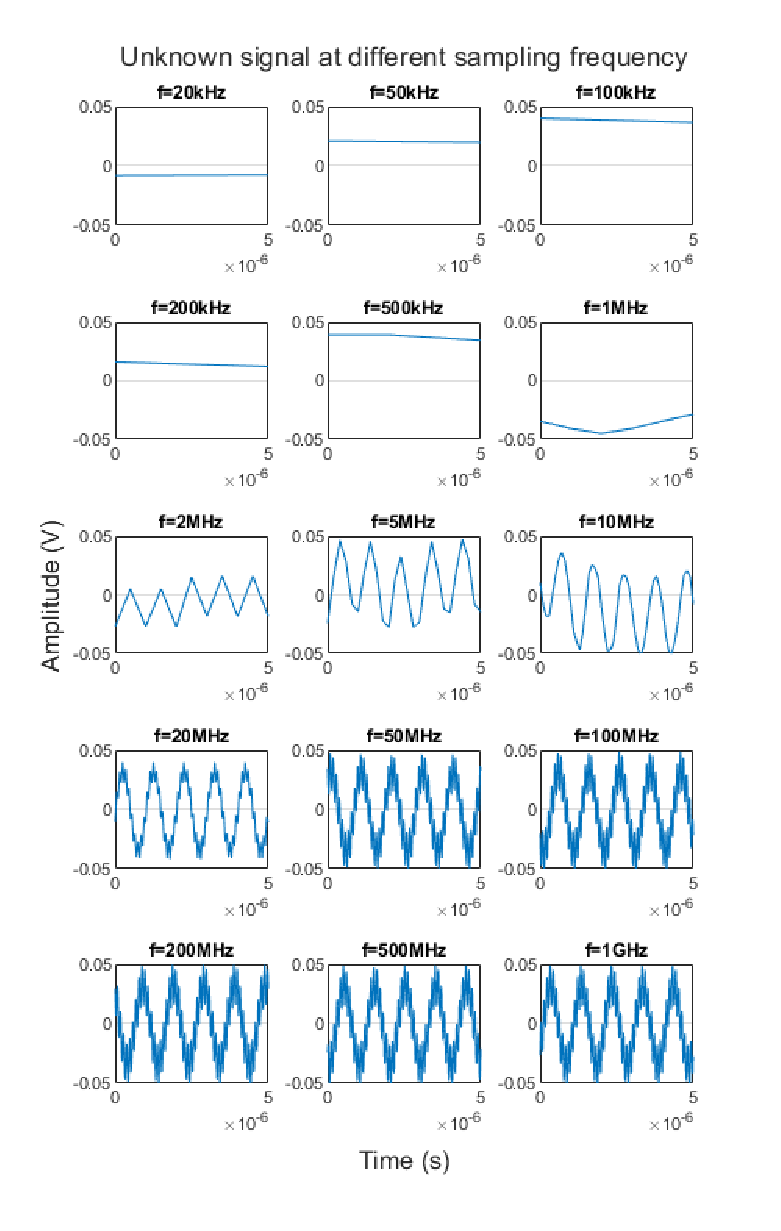
\includegraphics[width=\maxwidth{50.17561465127948em}]{figure_4.eps}
\end{center}

\begin{par}
\begin{flushleft}
Plotting the 1 GHz plot alone 
\end{flushleft}
\end{par}

\begin{matlabcode}
figure()
plot(T3.t28, T3.D28)
title("Unknown Signal at a Sampling Frequency of 1GHz")
grid("on")
xlim([0, 3e-6]);
ylim([-0.05, 0.05]);
\end{matlabcode}
\begin{center}
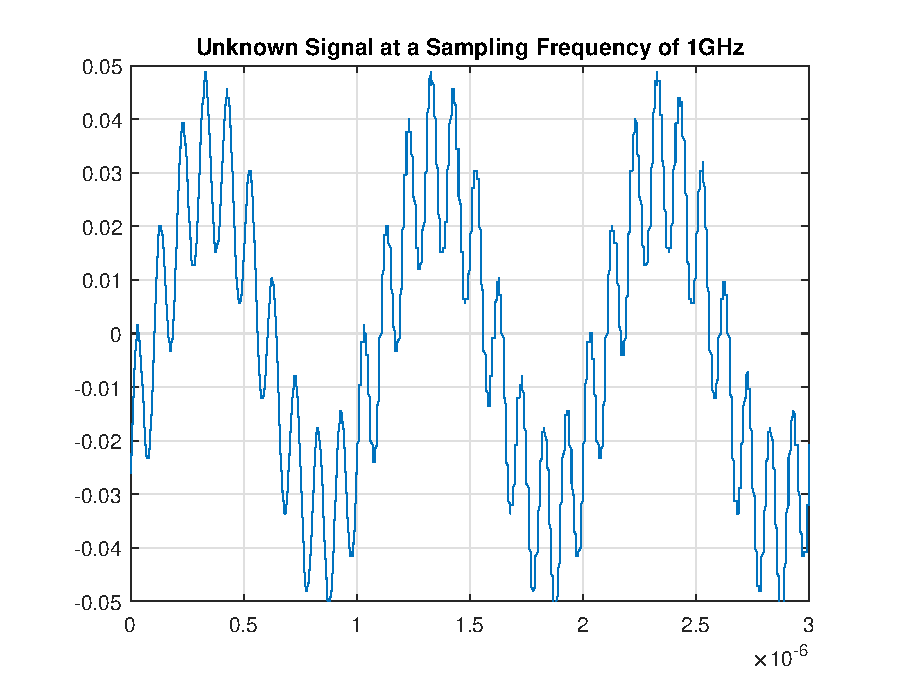
\includegraphics[width=\maxwidth{56.196688409433015em}]{figure_5.eps}
\end{center}

\begin{par}
\begin{flushleft}
Finding FFT of the unknown signal
\end{flushleft}
\end{par}

\begin{matlabcode}
Y = fft(T3.D28);
Fs = 1e9;
L = length(T3.D28);
figure()
plot(log10(Fs/L*(0:L-1)),abs(Y)/L,"LineWidth",3)
title("FFT of the unknown signal")
xlabel("log10(f) (Hz)")
ylabel("|fft(X)|")
xlim([5,10]);
ax = gca;
chart = ax.Children(1);
datatip(chart,9,0.01669);
datatip(chart,7,0.008271);
datatip(chart,6,0.01669);
\end{matlabcode}
\begin{center}
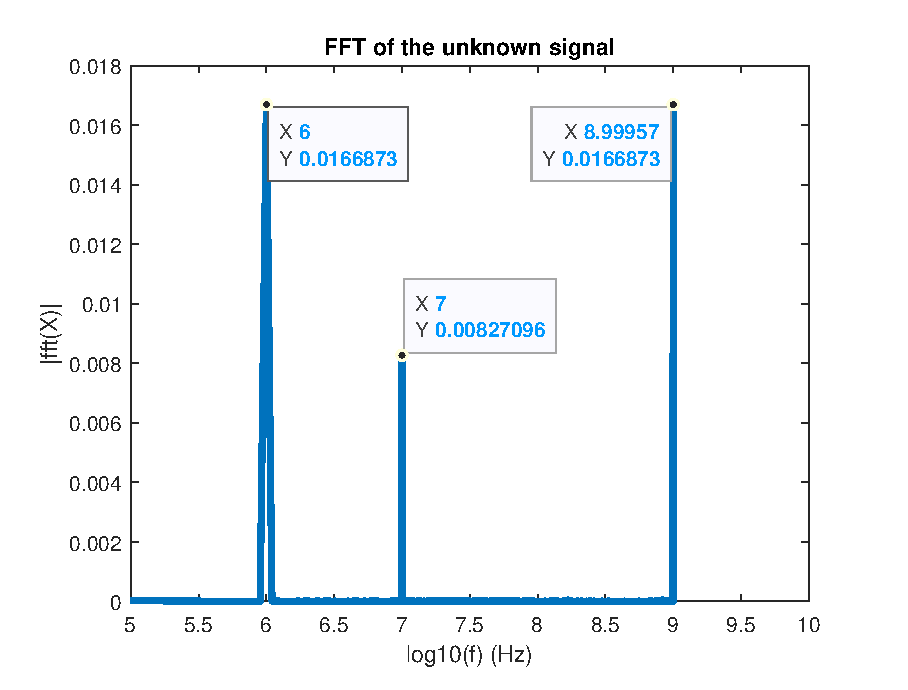
\includegraphics[width=\maxwidth{56.196688409433015em}]{figure_6.eps}
\end{center}
\begin{matlabcode}

\end{matlabcode}

\begin{par}
\begin{flushleft}
Verification of FFT results
\end{flushleft}
\end{par}

\begin{matlabcode}
figure()
time1=0:1e-11:5e-6;
X = mean(T3.D28)+0.01669*sin(2*pi*1e6*time1)+0.008271*sin(2*pi*1e7*time1)+0.01669*sin(2*pi*1e9*time1);
figure()
t = tiledlayout(3,1);
nexttile
plot(time1, sin(2*pi*1e6*time1))
title("f1 = 1MHz")
grid("on")
xlim([0, 3e-6]);

nexttile
plot(time1, sin(2*pi*1e7*time1))
title("f2 = 10MHz")
grid("on")
xlim([0, 3e-6]);

nexttile
plot(time1, sin(2*pi*1e9*time1))
title("f2 = 1GHz")
grid("on")
xlim([0, 1e-8]);

xlabel('Time (s)');
ylabel('Amplitude (V)');
title('Constituents of the unknown signal')
\end{matlabcode}
\begin{center}
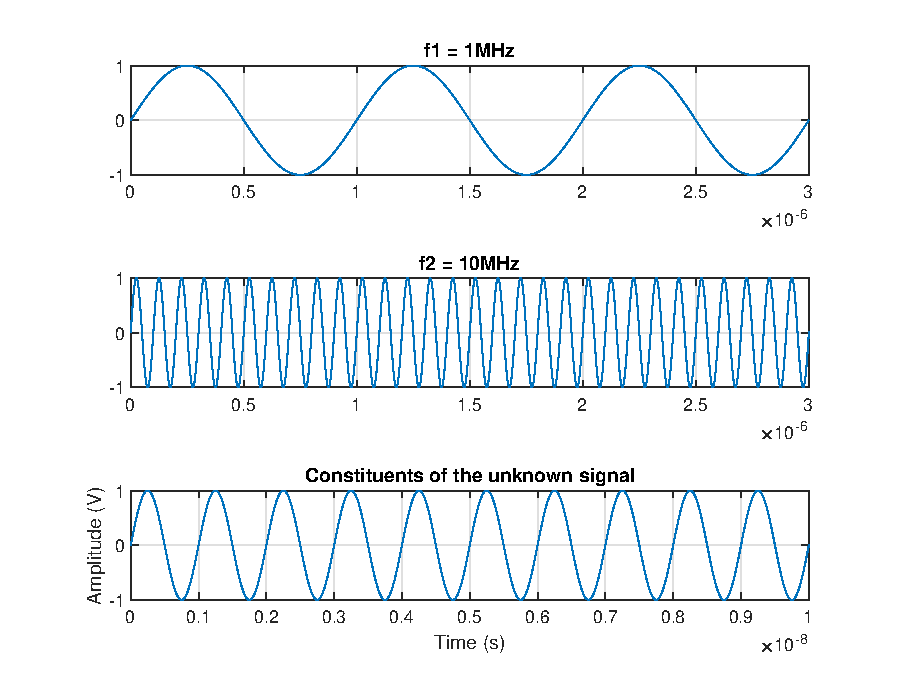
\includegraphics[width=\maxwidth{56.196688409433015em}]{figure_7.eps}
\end{center}


\vspace{1em}
\begin{matlabcode}
figure()
plot(time1, X)
title('Fourier Reconstruction of the unknown signal')
grid("on")
xlim([0, 3e-6]);
ylim([-0.05, 0.05]);
\end{matlabcode}
\begin{center}
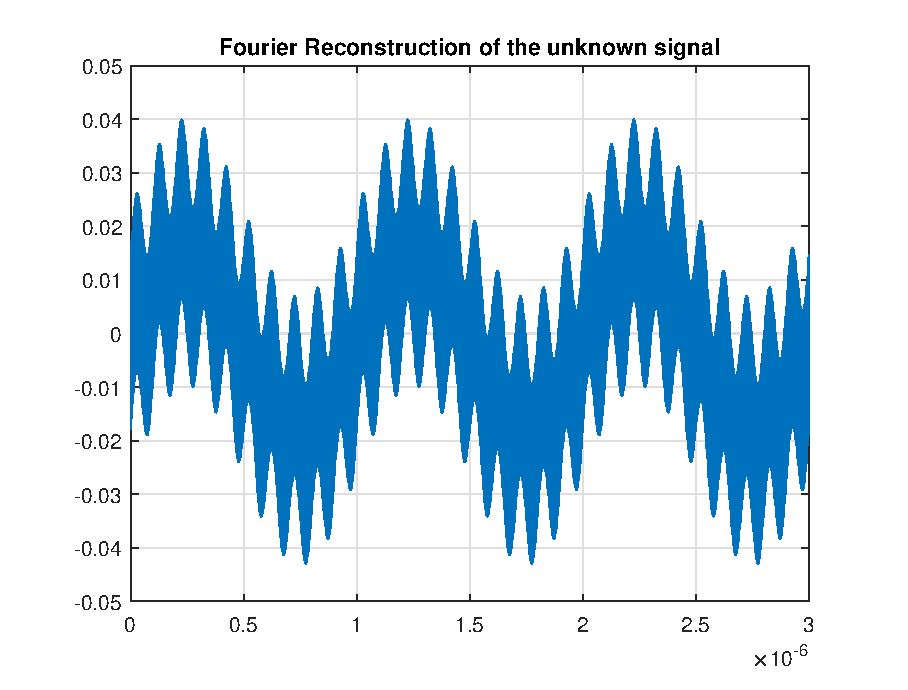
\includegraphics[width=\maxwidth{56.196688409433015em}]{figure_8.eps}
\end{center}

\end{document}
